\documentclass[aps,prx,10pt,twocolumn,floatfix,superscriptaddress,showpacs,numerical,footinbib]{revtex4-1}

\usepackage{graphicx}
\usepackage{amsmath}
\usepackage{amssymb}
\usepackage[T1]{fontenc}
\usepackage[utf8]{inputenc}
\usepackage{hyperref}
\usepackage[pdftex]{color}

\newcommand{\sgn}[1]{\mathrm{sgn} \left( #1 \right)}
\newcommand{\e}{\mathrm{e}}
\newcommand{\im}{\mathrm{i}}
\newcommand{\di}{\mathrm{d}}
\newcommand{\ket}[1]{| #1 \rangle}
\newcommand{\bra}[1]{\langle #1 |}
%\renewcommand{\thefootnote}{\fnsymbol{footnote}}

\newcommand{\noteAG}[1]{{\color{blue} [AG: #1]}}
\newcommand{\noteFP}[1]{{\color{magenta} [FP: #1]}}
\newcommand{\noteJM}[1]{{\color{red} [JM: #1]}}
\newcommand{\noteFdJ}[1]{{\color{cyan} [FdJ: #1]}}
\newcommand{\bs}[1]{{\boldsymbol{#1}}}


\begin{document}
%
\title{Interaction driven phases in the half-filled honeycomb lattice: an infinite density matrix renormalization group study}
%
%\author{Johannes Motruk}
%\author{Adolfo. G. Grushin}
%\affiliation{\mbox{Max-Planck-Institut f\"ur Physik komplexer Systeme, N\"othnitzer Str.\ 38, 01187 Dresden, Germany}}
%\author{Fernando de Juan}
%\affiliation{\mbox{Materials Science Division, Lawrence Berkeley National Laboratories, Berkeley, CA 94720, USA}}
%\affiliation{\mbox{Department of Physics, University of California, Berkeley, CA 94720, USA}}
%\author{Frank Pollmann}
%\affiliation{\mbox{Max-Planck-Institut f\"ur Physik komplexer Systeme, N\"othnitzer Str.\ 38, 01187 Dresden, Germany}}
%
\date{\today}
%
\begin{abstract}
%
%
The emergence of the Haldane Chern insulator state due to strong short range electron-electron interactions in the half-filled spinless honeycomb lattice
model has been proposed and challenged with different methods.
%
In this work we revisit the problem using the infinite density matrix renormalisation group method to go beyond previous mean field theory and exact
diagonalization studies.
%
We report numerical evidence supporting 
i) the absence of the Chern insulator state, 
ii) two previously unnoticed charge ordered phases, 
iii) the existence and stability of all the non-topological competing orders that were found previously within mean field and
iv) the character of the relevant phase transitions.
%
Our work establishes the phase diagram of the half-filled honeycomb lattice model tilting the balance
towards the absence of Chern insulator phase for this model.
%
%\noteAG{There are specific commands to leave comments like this one}\noteFP{or this}\noteJM{or this}\noteFdJ{or this}
%
\end{abstract}
%
\maketitle
%

\section{Introduction}
%
Topological phases of matter are remarkably robust states; their responses to external fields are
governed by topological invariants and thus many of their most important properties are insensitive to local perturbations~\cite{HK10,QZ11}.
%
Topologically protected responses result in intrinsically novel phenomena
including fractionalization of quantum numbers~\cite{Nayak2008} or transport governed by quantum anomalies~\cite{V03}
and can lead to diverse applications, ranging from fault tolerant quantum computation to spintronics~\cite{HK10,QZ11,Nayak2008}.
%
Added to the remarkable experimental discoveries of new topological phases in both two and three dimensions,
these ideas have boosted a sustained and voluminous scientific effort in the last decade that attempts to classify them 
and determine when and how can they emerge~\cite{S14}.\\
%

This work is embedded in the latter problem and concerns a concrete question that has so far
remained controversial: the existence of the Chern insulator phase triggered by short-range electron-electron interactions in the
spinless half-filled honeycomb tight binding model.
%
The Chern insulator state, first identified by Haldane~\cite{H88} in the particular case of the honeycomb lattice, is a zero field analogue of the
integer quantum Hall effect; the Hall conductivity contribution of each band is quantised in integer units of $e^2/h$ and determined by a topological invariant, the Chern number.
%
Realising a Chern insulator in nature is not a trivial task~\cite{CZF13}; time-reversal must be broken with
the resulting magnetic flux averaging to zero over the unit cell, and thus over the entire sample.
%
In a remarkable proof of principle, a set of mean field studies~\cite{RQHZ08,WF10,GCC13} discussed how the Chern insulator can 
occur from electron-electron interactions. 
%
It was shown that spinless electrons hoping in the half-filled honeycomb lattice with nearest and next-to-nearest neighbour interactions, $V_{1}$ and $V_{2}$ respectively, 
displayed a Chern insulator phase as described by Haldane.
%
This particular realization of the Chern insulator phase has complex nearest neighbour hopings [see Fig.~\ref{fig:orders}(g)]
and therefore within the mean field paradigm occurs in the region where $V_{2}>V_{1}$.
%
The latter condition 
was shown not to be a generic requirement; Chern insulator phases can be realized 
in mean field with only $V_{1}$ at the expense of enlarging the unit cell and doping the system~\cite{CGV11,GCC13}.
%
In addition, analogous topological phases have been obtained in other lattices such as the square lattice~\cite{WF10,JGC13}.
%
\begin{figure}
%
 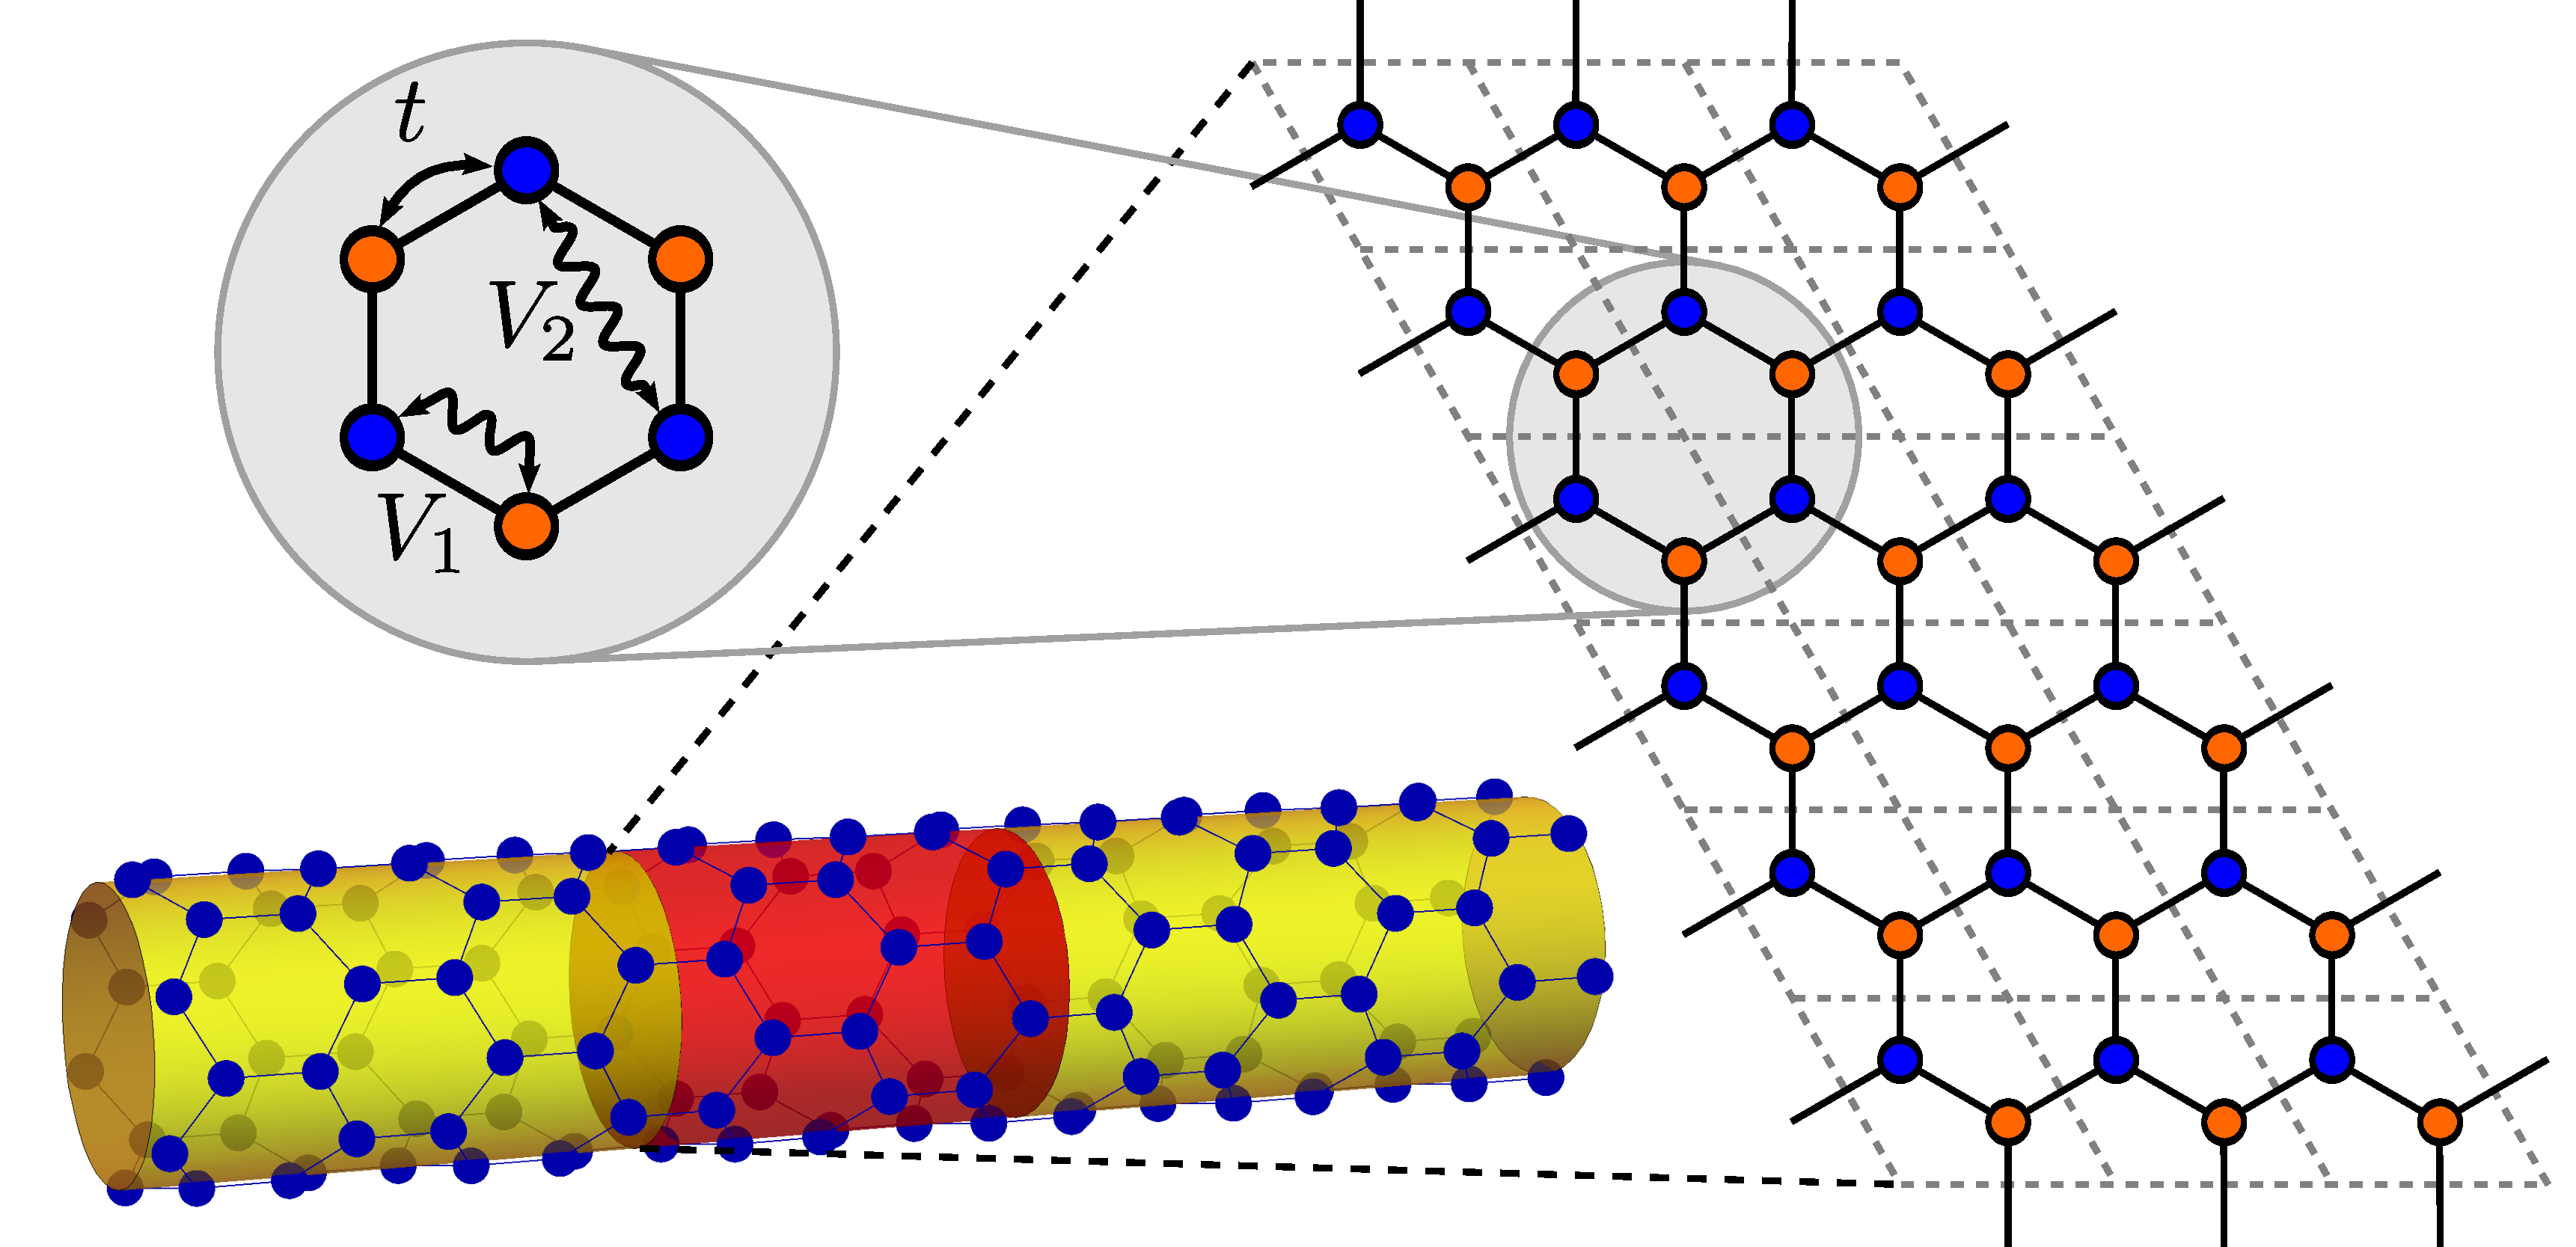
\includegraphics[width=\columnwidth]{pdf/unit_cell.pdf}
 %
 \caption{The upper panel shows a schematic representation of the interacting tight binding model considered in this work:
 %
fermions hoping in a half-filled honeycomb lattice with nearest-neighbour hopping $t$ (full lines) and interacting via
 nearest and next-to-nearest neighbour interactions, $V_{1}$ and $V_{2}$ respectively (dashed lines) as defined by 
 \eqref{eq:H}.
 %
 The left panel shows the iDMRG unit cell used in this work with 
 $3 \times 6$ unit cells yielding a cylinder with a circumference of $L=12$ sites depicted in the lower panel. 
 %
 \label{fig:Defs}}
\end{figure}
%% 
\\

The important question that still remains to be answered is wether the interaction induced Chern state survives 
after the effect of quantum fluctuations is included.
%
The Haldane Chern insulator phase competes with more conventional but also interesting orders, 
that can jeopardise its emergence and are depicted schematically in Fig.~\ref{fig:orders}.
%
On the one hand, in the $V_{1} \gg V_{2}$ limit, a charge ordered state depicted in Fig.~\ref{fig:orders}(b) is expected, 
where the A and B sub lattices are populated differently~\cite{RQHZ08,WCT14} \noteAG{cite Monte Carlo refs}.
%
Being connected to the classical ground state at $V_{1}/t \to \infty$ with only one occupied sublattice, this state (CDW-I) has been found to be very robust both in mean field an exact diagonalization.
%
For $V_{2}\gg V_{1}$ on the other hand it was shown under the mean field paradigm~\cite{GCC13} that the phase space originally attributed to the Haldane Chern insulator 
was severely reduced by the presence of a sublattice charge modulated state (or CMs) depicted in Fig.~\ref{fig:orders}(c).
%
The CMs phase was corroborated to survive quantum fluctuations in exact diagonalization~\cite{GGNVC13,DCH14} and within a variational Monte Carlo approach~\cite{DCH14}.
%
However, its exact nature was questioned by Ref.~\cite{DH14} where it was argued that a pinball liquid state~\cite{HF06,MRF13} --a state where a fraction of electrons remains pinned to fixed lattice sites while the remaining fermions explore the unoccupied sites-- cannot be discarded. 
%
In addition, at intermediate $V_{1}\lesssim V_{2}$ a Kekul\'e bond order~\cite{C00,HCM07,WF10,RH10,RJH13} depicted in Fig.~\ref{fig:orders}(d), that triples the original honeycomb two atom unit cell, 
was found to be stable within mean field theory.
%
Although numerical evidence consistent with such bond order was found in exact diagonalization~\cite{GGNVC13}, further insights are needed to corroborate its existence in the thermodynamic limit.
%
Finally, the Haldane Chern insulator phase of Fig.~\ref{fig:orders}(g), stable within mean field, was found however to be absent in exact diagonalization with periodic boundary conditions~\cite{GGNVC13,DH14} and cluster perturbation theory~\cite{DH14} suggesting that quantum fluctuations indeed can destabilize its emergence.
%
Nonetheless, this interpretation was challenged by Ref.~\cite{DCH14} that observed hints of this phase with exact diagonalization with open boundary conditions and variational Monte Carlo.\\

%
%
\begin{figure}
 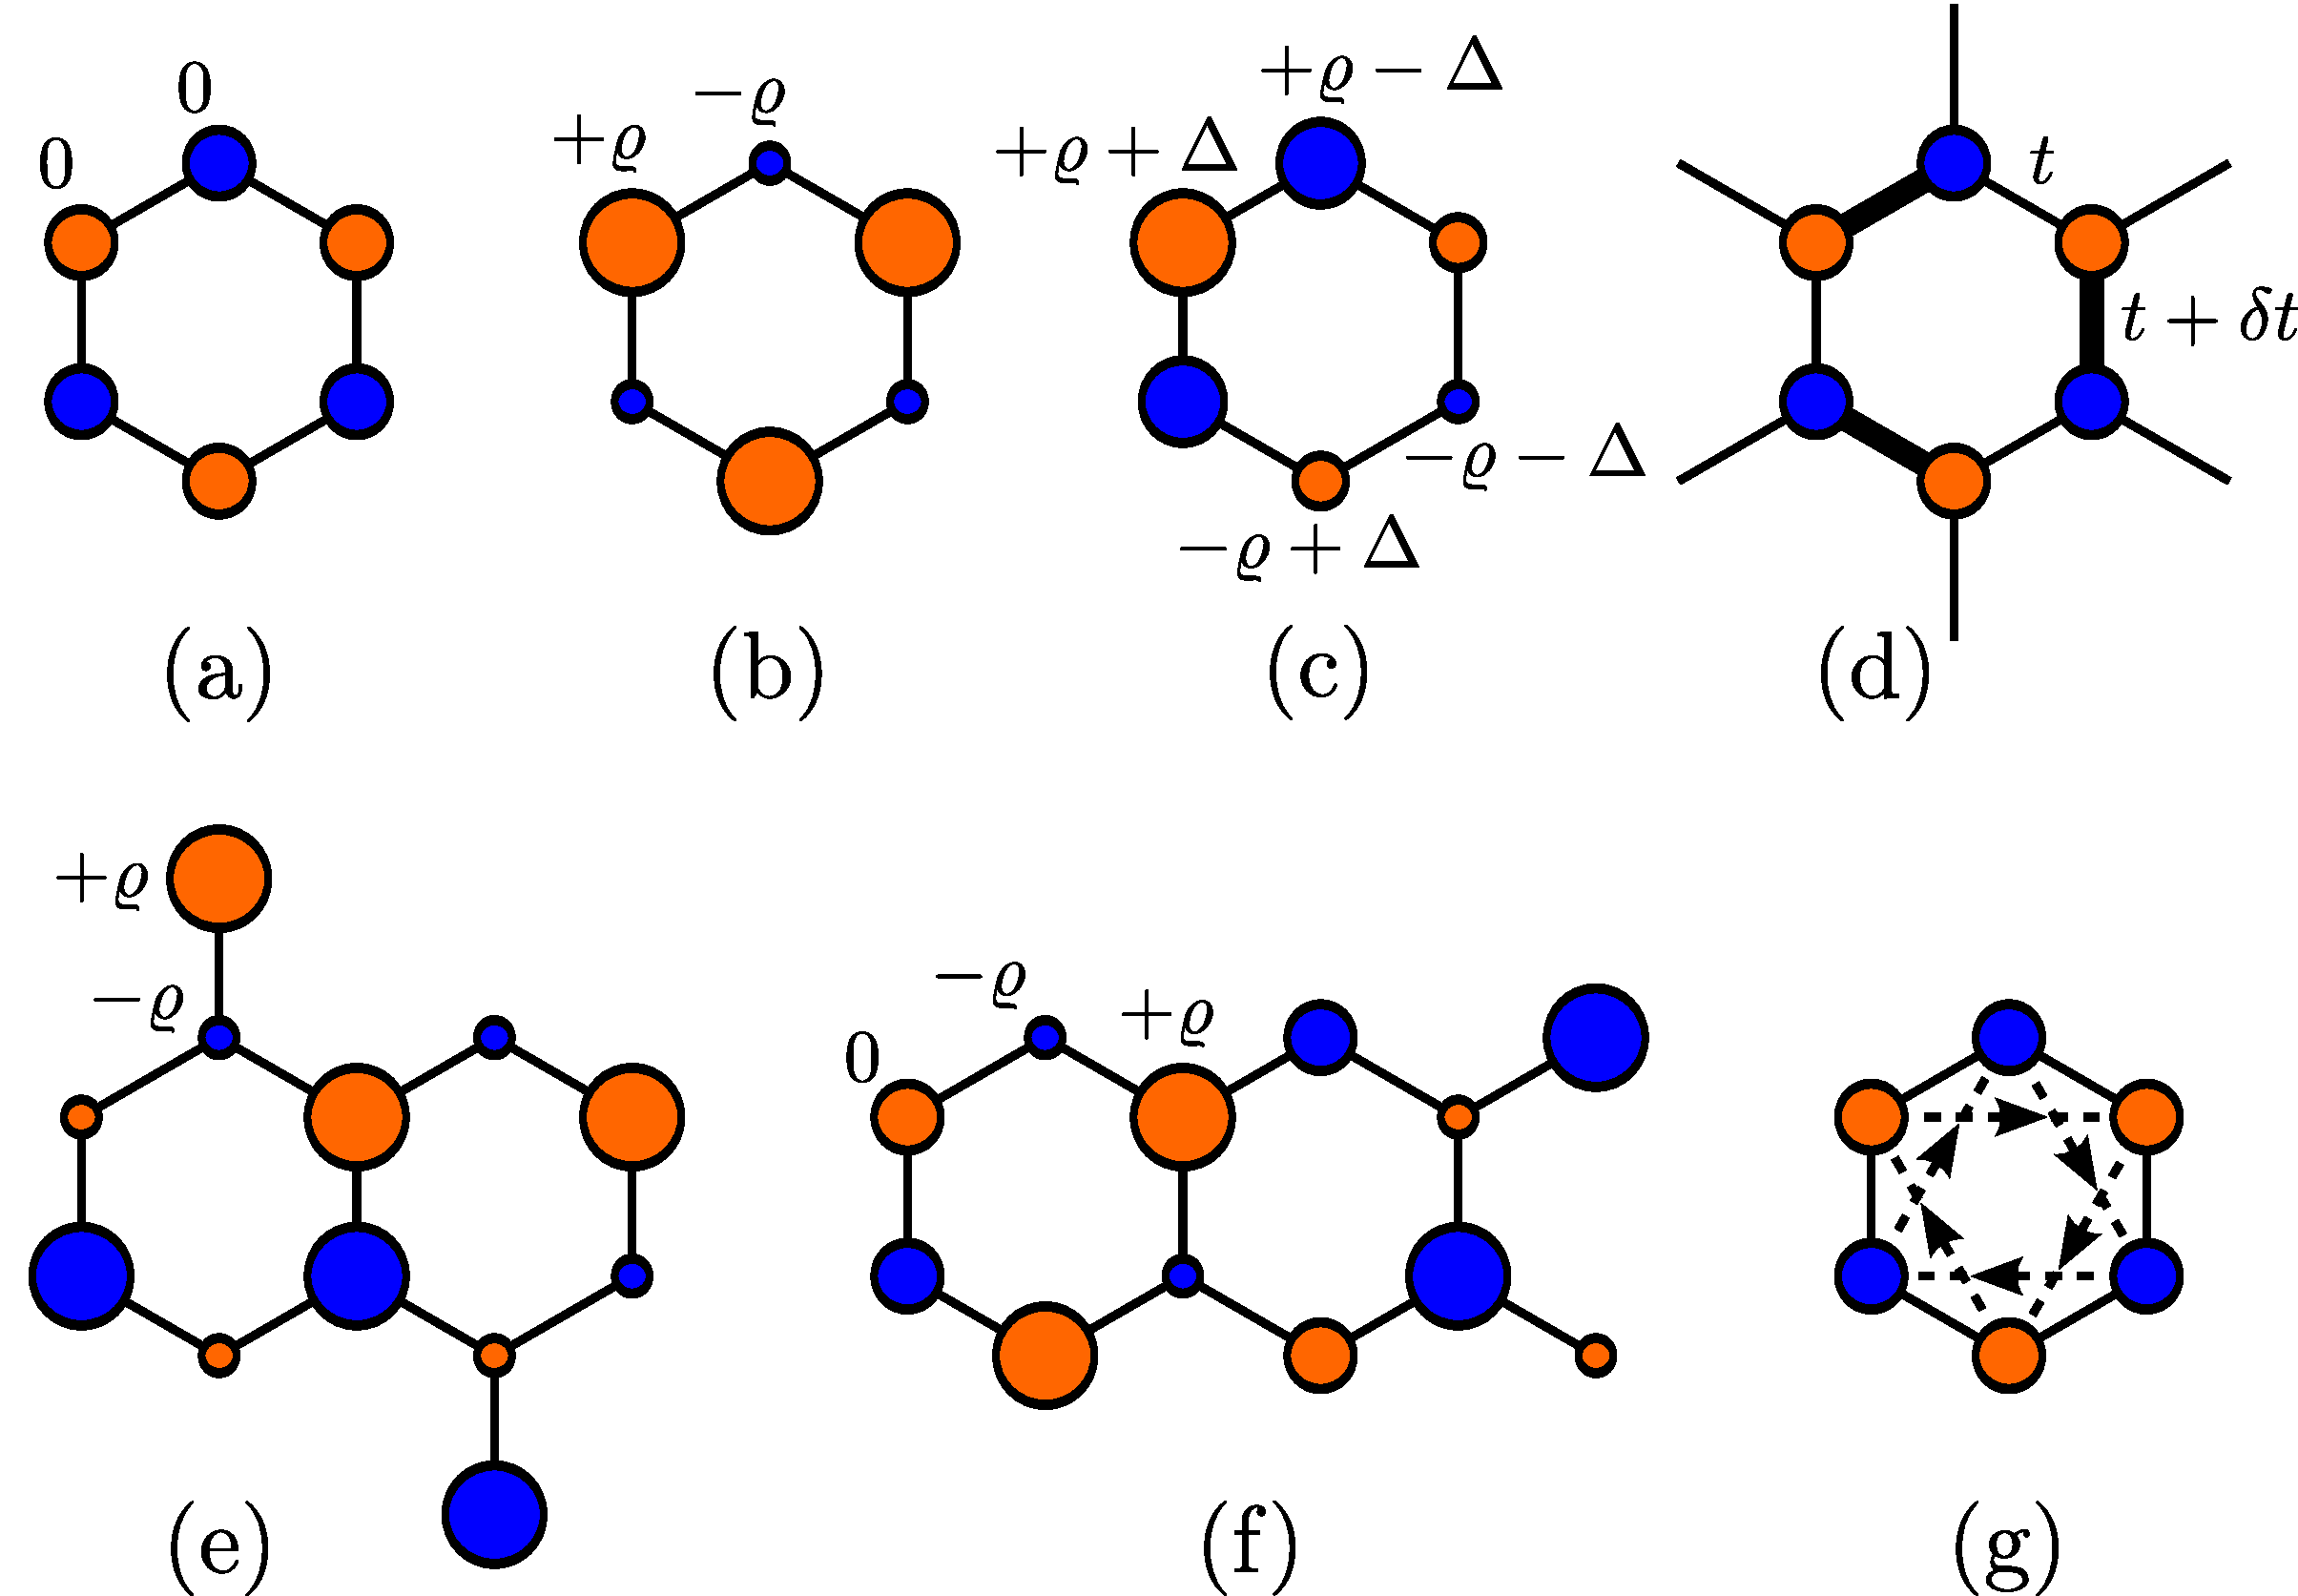
\includegraphics[width=\columnwidth]{{pdf/orders}.pdf}
 %
 \caption{Different orders allowed in the half-filled spineless Honeycomb lattice considered in this work:
 % 
 (a) Semimetal, (b) CDW I, (c) CMs, (d) Kekul\'e, (e) CDW II, (f) CDW III, (g) Haldane phase. 
 %
 Phases (a)-(d) and (g) were found within mean field theory by Refs.~\cite{RQHZ08,WF10,GCC13}.
 %
The survival of the Haldane Chern insulator phase (g) was challenged within exact diagonalization with periodic boundary conditions
by Refs.~\cite{GGNVC13,DH14} but found in Ref.~\cite{DCH14} for open boundary conditions.
 %
 The exact nature of phase (c) was questioned within exact diagonalization by Ref.~\cite{DH14}.
 %
 \label{fig:orders}}
 %
\end{figure}
%
The contradictory numerical evidence regarding the existence of the Chern insulator phase in particular, and other competing phases in general, needs of an alternative approach
that includes quantum fluctuations while minimizing finite size effects.
%
In this work we therefore revisit the controversies left unsolved by previous studies using the infinite density matrix renormalization group method (iDMRG)~\cite{M08,W92,KZM13}. 
%
This variational method determines the ground-state of systems of size $L_{x} \times L_{y}$ where $L_{x}$ is in the thermodynamic limit and $L_{y}$ goes beyond
what is achievable in exact diagonalization.
%
Traditionally a method for finding the ground state of one-dimensional systems, there has been recent 
important progress and reported success of iDMRG applied to two dimensional systems.
%
As long as entanglement remains low and the state has short correlation lengths the ground-state
can be represented faithfully by a product of matrices, termed matrix product state (MPS), with matrices of a finite and computationally affordable
dimension $\chi$~\cite{M08,W92,KZM13}.
%
This requirement is commonly met by gapped systems and in particular by the orders argued above to be expected instabilities in the half-filled 
honeycomb lattice of interest here.
%
Moreover the iDMRG deals with an infinite system and thus, unlike exact diagonalization, it can probe directly ground states that spontaneously break the original symmetries of the Hamiltonian and the phase transitions among them, while allowing for quantum fluctuations to play a role. 
%
Recently the infinite and finite DMRG method were indeed shown to be able to characterise the properties of fractional quantum Hall states~\cite{ZMP13},
$\mathbb{Z}_{2}$ quantum spin liquid~\cite{HSC14}, chiral spin liquid \cite{HSC14b} and bosonic and fermionic fractional Chern insulating states \cite{JWB12,CV13,ZKB13,GMZ15}.
\\
 
%
Motivated by these advantages we have mapped with the iDMRG method the $\left\lbrace V_{1},V_{2}\right\rbrace$ phase diagram for the half-filled honeycomb lattice in the infinite cylinder geometry.
%
Our main findings are summarised next.
%
First we show compelling numerical evidence that supports the absence of the Chern insulator state in a wide region of $\left\lbrace V_{1},V_{2}\right\rbrace$ phase space.
%
Second, we find two new phases not reported previously neither within mean field or exact diagonalization results and give a semiclassical argument for one 
of these to occur.
%
Third, we provide numerical support for the existence and stability of all the competing orders that were found previously within mean field.
%
In particular we characterise the two more controversial states, the CMs and Kekul\'{e} states, by computing bond and charge expectation values via the iDMRG method 
and present further arguments of the existence of the former from the semiclassical large interaction limit.
%
Fourth, we provide numerical evidence to asses the first or second order character of the relevant phase transitions.
%
Concretely we address this issue by identifying the features that the correlation length $\xi$ and the entanglement entropy $S$ present as a function of $\left\lbrace V_{1},V_{2}\right\rbrace$.\\

This work is structured as follows. 
%
After describing the method and model in section~\ref{sec:modandmeth} we
characterise the different phases that we find in section~\ref{sec:phasediagram}.
%
The different phase transitions among them are analyzed in section~\ref{sec:phasetransitions}
and we end with a discussion and prospect of our results in section~\ref{sec:discconc}.


\section{\label{sec:modandmeth}Model and Method}
%
We investigate a system of spinless electrons hopping on a honeycomb lattice with real nearest neighbor hopping $t$ interacting via nearest and next to nearest neighbor interactions 
$\left\lbrace V_{1},V_{2}\right\rbrace$ respectively [see Fig.~\ref{fig:Defs}]. 
%
The Hamiltonian for this system can be written as
 %
\begin{equation}
%
 H:=-t\sum_{\left\langle i,j\right\rangle}(c^{\dagger}_{i}c^{\vphantom{\dagger}}_{j}+ \mathrm{h.c.})+
 %
V_{1}\sum_{\left\langle i,j\right\rangle }n_{i}n_{j}+
%
V_{2}\sum_{\left\langle \left\langle i,j\right\rangle \right\rangle }n_{i}n_{j}.
%
\label{eq:H}
\end{equation}
%
where $c_{i}^{\vphantom{\dagger}}$ $(c^{\dagger}_{i})$  annihilates (creates) an electron at the $i$-th site of the honeycomb lattice.
% in sublattice $s=A,B$ and $s\neq\bar{s}$. 
%
% Each of the two triangular sublattices A and B is spanned by the basis vectors
% $\bs{a}_{1}=\bs{\delta}_{2}-\bs{\delta}_{3}$ and 
% $\bs{a}_{2}=\bs{\delta}_{3}-\bs{\delta}_{1}$ defined through the three nearest neighbors $\bs{\delta}_{1}=a(0,-1)$,  
% $\bs{\delta}_{2}=a(\sqrt{3}/2,1/2)$ and $\bs{\delta}_{3}=a(-\sqrt{3}/2,+1/2)$ as shown in Fig.~\ref{fig:Defs}.\\
%

In order to find the ground state of the system in the $\left\lbrace V_{1},V_{2}\right\rbrace$ phase space
we employ the infinite density matrix renormalization group algorithm (iDMRG) \cite{M08,W92,KZM13} on an infinite cylinder geometry.
%
Feasible system sizes for our purposes are cylinders of circumference $L = 6,8,10$ and $12$.
%
For our calculations we choose a unit cell of 36 sites depicted in Fig.~\ref{fig:Defs}.
%
It consists of three rings of 12 sites each wrapping around the cylinder.
%
We pick this geometry for the following two reasons.
%
First, all orders expected to occur in the half-filled honeycomb model are commensurate with the chosen unit cell.
%
Second, we have to keep in mind the structure of the reciprocal space.
%
Since we work in the thermodynamic in the $x$-direction along the cylinder, momentum in $x$-direction is a continuous quantity.
%
However in the $y$-direction around the cylinder, momentum is discretized.
%
In the non-interacting case, the model forms a Dirac semimetal with the Fermi surface consisting of the $K$ and $K^{\prime}$ points which possess momenta $k_y=k_y^{\prime} = 2\pi / 3$.
%
Any instability caused by interactions will open a gap at these points.
%
In order to  capture the low energy physics correctly, it is very important that $k_y= 2 \pi / 3$ is an allowed momentum in our unit cell.
%



\section{\label{sec:phasediagram}Phase diagram}
%
We have used the iDMRG method to find the groundstate of the half-filled honeycomb lattice in the presence of 
$\left\lbrace V_{1},V_{2}\right\rbrace$ interactions.
%
Our results are summarised in the phase diagram presented in Fig.~\ref{fig:phase diagram}.
%
As a function of $\left\lbrace V_{1},V_{2}\right\rbrace$ we find six different phases, 
including two novel charge order phases (CDW-II and CDW-III) together with the previously 
reported mean field orders: Kekul\'{e}, CMs, CDW-I and semimetal phases.\\
%
%
Within the iDMRG algorithm we have computed the charge and bond ground state expectation values
to characterise each phase.
%
At each site the charge expectation value is defined by 
%
\begin{eqnarray}
\label{eq:charge}
n_{i,s}=\left\langle c^{\dagger}_{i,s}c_{i,s}\right\rangle,  
\end{eqnarray}
%
where $s=A,B$ is the sublattice index. 
%
The bond ground state expectation value on the other hand is defined as
%
\begin{eqnarray}
\label{eq:bond}
t^{s,s'}_{i,j}=\left\langle c^{\dagger}_{i,s}c_{j,s'}\right\rangle.
\end{eqnarray}
%
%
We describe next the corresponding charge and bond ordering patterns of each phase 
that characterise them within the iDMRG method.

\begin{figure*}
 
\includegraphics[width=\textwidth]{pdf/phase_diagram_ext.pdf}
 \caption{Left: Phase diagram obtained with iDMRG calculations on an infinte cylinder of circumference $L=12$. 
 %
 Right: Density ((a)--(d)) and hopping amplitude ((e)--(h)) patterns in the different phases. 
 %
 The area of the blue circles is proportional to the particle number expectation value on the respective site. 
 %
 The thickness of the ellipsoids on the bonds is proportional to the hopping amplitude $t_{ij}$ \eqref{eq:hop} between nearest neighbours.
 %
 The unit cells are depicted by the red polygons. 
 %
 ((a)/(e)) Charge modulated (CMs) phase with $V_1/t = 0.8, V_2/t = 3.2 $, ((b)/(f)) Charge density wave II (CDW II) with $V_1/t = 5.6, V_2/t = 3.2$,  ((c)/(g)) Charge density wave III (CDW III) with $V_1/t = 9.2, V_2/t = 2.5$, ((d)/(h)) Kekul\'e phase with $V_1/t = 5.6, V_2/t = 1.6 $. 
 \label{fig:phase diagram}}
\end{figure*}


%
\subsection{Semimetal phase (SM)}
%
We start by discussing the semimetal phase, labelled SM in the phase diagram shown in Fig.~\ref{fig:phase diagram}.
%
At $V_{1}/t=V_{2}/t=0$ the honeycomb lattice with nearest neighbour hopping its 
known to be described by a low energy theory in terms of two massless Dirac fermions~\cite{CastroNeto2009}.
%
Upon including finite short range interactions, it is possible to show that these are irrelevant in the renormalisation group sense~\cite{S94,KUP12} 
and therefore they can only drive a transition to an ordered state when they have a magnitude comparable to the nearest neighbour hopping strength $t$.
%
Such perturbative analysis guarantees that the semimetal is stable within
the region $\left\lbrace V_{1},V_{2}\right\rbrace \lesssim t$, only allowing for a uniform renormalization 
of the hopping strength $t$ by interactions.\\

%
For the SM phase in Fig.~\ref{fig:phase diagram}, and to numerical accuracy, we find by computing the charge expectation value
\eqref{eq:charge} that $n_{i,A}=n_{i,B}=1/2$, indicating that this phase is not charge ordered.\\
%
From \eqref{eq:bond} and choosing $i,j$ to be nearest neighbours we find
a small ($\sim10^{-2}$) asymmetry between bonds pointing along and around the cylinder axis.
%
Such asymmetry should vanish in a perfect semimetallic phase and indeed it is severely reduced as the bond dimension $\chi$ is increased.
% 
This suggests that the cylinder geometry implemented in iDMRG artificially differentiates bonds in its two perpendicular directions,
since it vanishes as $\chi$ is increased, and is not a physical effect.
%
This is consistent with a semimetal state, since the logarithmic divergence of entanglement of a metallic state requires an matrix product state with $\chi\to\infty$. 
%
The bond asymmetry reduces the entanglement by shifting the Dirac cones away from the $\mathbf{K}$ and $\mathbf{K'}$ points~\cite{ACJ15}.
%
In addition, we find as well that the bond strength increases with interaction strength, as expected form the renormalisation group analysis. \\
%
Together, the previous numerical evidence is consistent with the semimetallic state.
%
We note that numerically this state seems to extend beyond $\left\lbrace V_{1},V_{2}\right\rbrace \lesssim t$ towards
higher interaction strengths through a narrow SM trench in the phase diagram.
%
The size of this region at $L=6$ (not shown) suggest that it is likely to shrink as the circumference of the cylinder is increased but
a definitive statement requires going beyond the numerically accessible sizes. 
%

\subsection{Charge density wave (CDW-I)}
%
Upon increasing $V_{1}$ we identify a charge density wave state labelled CDW-I in the phase diagram of Fig.~\ref{fig:phase diagram}.
%
This state has a two site unit cell that is characterized by a finite order parameter
%
\begin{equation}
\label{eq:CDW}
%
M=\left\langle n_{A} \right\rangle-\left\langle n_{B}\right\rangle,
%
\end{equation}
%
that can be calculated using \eqref{eq:charge}, where $n_{A}$ and $n_{B}$ are the density of electrons in the $A$ and $B$ sublattice sites of the two site unit cell respectively.
%
The resulting charge order is depicted schematically in Fig.~\ref{fig:orders}(b).
%
For instance, at $V_{1}/t = 4$ and $V_{2}/t = 0.4$ we find that $M=$. \noteAG{I mention this as an example since we don't show the order, I don't know}
%
Numerically the magnitude of $M$ increases with $V_{1}$ and to numerical accuracy this phase has no appreciable bond order.\\
%s
For large $V_{1}\gg t$ such a state is a natural instability since the energy is minimised by a charge imbalance between the two sub lattices.
%
Indeed, it has been found in a mean field approximation~\cite{RQHZ08,WF10,GCC13}, exact diagonalization~\cite{GGNVC13,DH14,DCH14}, 
and quantum Monte Carlo simulations~\cite{WCT14}.
%


\subsection{Sub-lattice charge modulated phase (CMs)}
%
For large $V_{2}\ll t$ the ground state is classically degenerate. 
%
Within mean field it was shown that as long $V_{2}>V_{1}$
the system chose a charge ordered pattern with charge modulation over different sub lattices, termed the CMs phase~\cite{GCC13}.
%
Such order, schematically shown in Fig.~\ref{fig:orders}(c), has a six site unit cell, and minimises the large cost
attributed to $V_{2}$ by reversing two nearest neighbour dimers at the expense of paying the small energetic cost
determined by $V_{1}$.
%
Within exact diagonalization it has been argued that the CMs state survives quantum fluctuations~\cite{GGNVC13,DH14,DCH14} 
but its single particle nature was challenged in Ref.~\onlinecite{DH14} suggesting that a pinball like state~\cite{HF06,MRF13} cannot be ruled out.\\
%
With the iDMRG method we find that the CMs appears directly above the semimetallic phase~[see Fig.~\ref{fig:phase diagram}] .
%
A sample of the six site unit cell charge and bond pattern obtained from \eqref{eq:charge} for $V_1/t = 0.8, V_2/t = 3.2 $ is shown in Fig.~\ref{fig:phase diagram}(a).
%
Such pattern, survives in the region labelled CMs of the phase diagram and coincides with that obtained within mean field theory~\cite{GCC13} 
depicted schematically in Fig.~\ref{fig:orders}(c).
%
We note that the bond ordering of this phase is associated to the charge order 

% 
Moreover, we now show that the CMs state is expected from a semi-classical analysis as well.
%
For instance, for a given cluster, it is possible to find the number and energy of all the degenerate classical states, assuming $V_{2}\gg t$.
%
Within this approach, the hopping can be introduced as a perturbation $t$ to find how the degeneracy is lifted.
\noteAG{Maybe Fernando can rewrite these two paragraphs better. We may want to be more specific about order parameters etc.} 


\subsection{Kekul\'{e} bond order}
%
The next phase we identify is the Kekul\'{e}
bond order.
%
Like the CMs, it has a six site unit cell depicted schematically in Fig.~\ref{fig:orders}(d)
with uniform charge order and strong and weak bonds.
%
Under the mean field approximation the state arises between the CMs and the CDW-I state.
%
Although in exact diagonalization hints of this state are also observed,
the evidence supporting its occurrence is far from conclusive~\cite{GGNVC13} since
its tripled unit cell turns the analysis of larger clusters problematic.
%

Within iDMRG we find that these state is stable in a smaller but finite region compared to both 
exact diagonalization and mean field.
%
We show the state's numerically obtained charge and bond order patterns in Fig.~\ref{fig:phase diagram}(e) and (d) 
calculated with \eqref{eq:charge} \eqref{eq:bond} respectively.
%
The state has indeed two types of bonds (weak and strong) arranged as in Fig.~\ref{fig:orders}(d) 
and no charge order.
%
For instance for $V_{1}/t=$ and $V_{2}/t=$



\subsection{Charge density wave - II (CDW-II)}
%
All phases that we have described so far do not differ
from those predicted by mean field and exact diagonalization.
%
At high $V_{2}$ but with sufficiently large $V_{1}$ we observe that
a twelve site unit cell charge order (CDW-II) depicted schematically in 
Fig.~\ref{fig:orders}(e) emerges.
%
A sample of its charge and bond order, as obtained with iDMRG via \eqref{eq:charge} and \eqref{eq:bond} is
shown in Fig.~\ref{fig:phase diagram} (b) for $V_{1}/t=$ and $V_{2}/t=$.
\\
%

A strong coupling analysis performed in 12 site cluster with the shape of the CDW-II unit cell reveals a set of 8 classical states with the same charge pattern but classical occupations 0 or 1. 
%
The energy per site of these states does not have first order hopping corrections,
$E_{CDW-II} = V_2/2+V_1/4 + O(t^2)$, so the CDW-II is a stable strong coupling phase. 
%
As long as the cluster allows for this charge pattern, it must be present at sufficiently high $V_{1,2}$.
%
In fact, the energy of this classical state is always lower than that of the classical CM states, and it is only for low $V_1$ that the quantum corrections make the CM state favored. 
%

\subsection{Charge density wave - III (CDW-III)}
%



\section{\label{sec:phasetransitions} Phase transitons}
%
A crucial advantage of the iDMRG method is that, unlike finite
size methods such as exact diagonalization it can characterize the order of phase transitions.
%
In order to unravel the character of the phase transitions between
the phases described above we now study two quantities that are sensitive
to a phase change, the entanglement entropy $S$ and the correlation length $\xi$.
%
In Fig.~\ref{}  and Fig.~\ref{} we show how these quantities change along
the horizontal and vertical cuts depicted in Fig.~\ref{fig:phase diagram} respectively.
%

\subsection{Cut A: SM--CDW-I}

The first horizontal cut, labelled A addresses the character of the phase transition between the semi-metallic
phase and the simplest charge density wave (CDW-I) by fixing $V_{2}=0$.
%
This phase transition has been previously addressed with the quantum Monte-Carlo method~\ref{WCT14} 
and was determined to be of second order character.
%
The transition point with divergent correlation length was determined to be at $V_{1}=$ via finite size scaling.
\noteAG{need number and polishing, Johannes?}
%
In Fig.~\ref{fig:cut_V2_0} we show the correlation length as a function of $V_{1}$ 
for different values of the bond dimension $\chi$ and cylinder with $L=12$ circumference.
\begin{figure}
 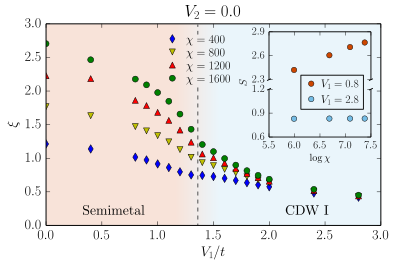
\includegraphics[width=\columnwidth]{{pdf/plot_cut_V2_0}.pdf}
 \label{fig:cut_V2_0}
 \caption{Correlation length at $V_2=0$. \noteFdJ{Perhaps add: Cut A in fig. 3. Since sections are labeled by the cuts, it could be useful to do this for every figure that represents a cut of fig. 3}  \noteAG{could it be useful to show the order parameter M
 as a function of $V_{1}$ in the same plot (using the right vertical axis?). It might get to crowded)}}
\end{figure}
% 
%
Firstly, for $V_{1}\leq 1.5t$ we observe that the correlation length diverges as the bond
dimension of the MPS is increased.
%
This behaviour is expected for a critical state such as the semimetal phase;  
the logarithmic divergence of entanglement of a metallic state requires an MPS with $\chi\to\infty$.
%
For $V_{1}\geq 1.5t$ the correlation length drops significantly and has no longer a significant 
dependence on $\chi$.
%
This is characteristic of a gapped phase such as the charge density wave.
%
The crossover is smooth, signalling a second order phase transition, in agreement with 
quantum Monte Carlo studies.
%
With iDMRG it is however not possible to pin point the exact value of $V_{1}$ 
where the transition happens via finite size scaling due to the few cylinder sizes 
we have available, as discussed in section \ref{sec:modandmeth}.
%
However, from Fig.~\ref{} it is however possible to define a crossover region $1.4 \lesssim V_{1}\lesssim 2$, 
\noteAG{this region ideally should coincide with color coding in the figure}
consistent with the quantum Monte Carlo data, where the transition occurs.

\subsection{Cut B: SM--CMs}
%
The cut at $V_{1}=0.4$, labelled cut B in Fig.~\ref{fig:phase diagram}, 
probes the transition between the semimetal phase and the CMs phases.
%
In Fig.~\ref{fig:cut_V1_0.4} we present the entanglement entropy $S$ as a function of $V_{2}$
, the interaction that drives the phase transition.

\begin{figure}
 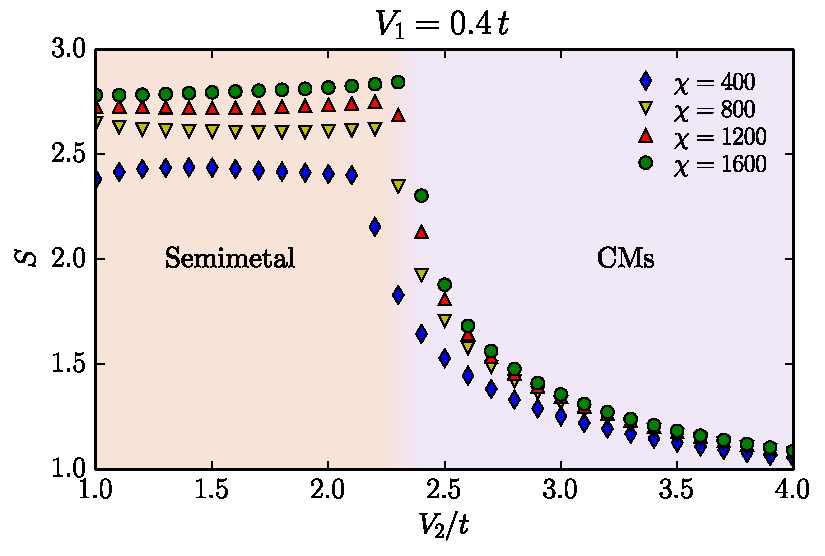
\includegraphics[width=\columnwidth]{{pdf/plot_cut_V1_0.4}.pdf}
 \caption{Entanglement entropy at $V_1=0.4$. \label{fig:cut_V1_0.4}}
\end{figure}
%
As expected from the previous analysis the entanglement entropy of 
the semimetal phase depends strongly on the MPS bond dimension $\chi$.
%
At $V_{2}\approx $ \noteAG{need value} we observe a sharp transition
to a decaying entanglement entropy that does not depend strongly on $\chi$
as $V_{2}$ is increased from the transtion.
%
This evidence is suggestive of a first order phase transition between
the semimetal and CMs phases.
%
The correlation length (not shown) also shows a discontinuity but not
as pronounced as the entanglement entropy.
%
\noteAG{Do we have an idea of why $S$ is better than $\xi$ sometimes to show phase transitions?}

\subsection{Cut C: CMs--CDW-II}

In cut C we fix $V_{2}=3.6$ and study the phase transition between
the CMs and the CDW-II phases.
%
The entanglement entropy is shown in Fig.~\ref{fig:cut_V2_3.6} 
as a function of $V_{1}$.
\begin{figure}
 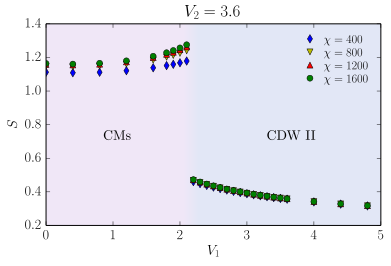
\includegraphics[width=\columnwidth]{{pdf/plot_cut_V2_3.6}.pdf}
 \caption{Entanglement entropy at $V_2=3.6$. \label{fig:cut_V2_3.6}}
\end{figure}
% 
%
This quantity shows a clear jump at $V_{2}\approx$ signalling a direct first order
phase transition between these two phases.
%

A first order phase transition is also expected from the strong coupling approach (see appendix). As described in section \ref{}, the energy per site of the CM phase in a 3x3 cluster is $E_{CM} = V_2/2+V_1/3$ for $V_1/V_2<3/2$, while the energy per site of the CDW II phase is $E_{CDW II} = V_2/2+V_1/4$. At $t=0$, $V_1=0$ both states have the same energy. At finite $t$, the CM phase has lower energy due to the first order quantum correction, which is absent for CDW II. But since $E_{CM}$ grows faster with $V_1$ than $E_{CDW II}$, there must be a crossing at a critical $V$ signaling a first order phase transition into the CDW II state. 

\noteAG{Is this expected semi-classically somehow?}\noteFdJ{Yes}

\subsection{Cut D: CDW-I--Kekul\'{e}--SM--CDW-II}

\begin{figure}
 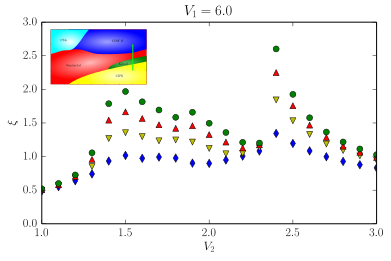
\includegraphics[width=\columnwidth]{{pdf/plot_cut_V1_6}.pdf}
 \caption{Correlation length at $V_1=6$. \label{fig:cut_V1_6}}
\end{figure}


\subsection{Cut E: SM--CDW-III}





% 




%
\section{\label{sec:discconc}Discussion and Conclusions}
%

The spontaneous emergence of the Chern insulator phase due to interactions in the half-filled spineless honeycomb lattice
model has been questioned by different methods since its proposal~\cite{RQHZ08,WF10,GCC13,GGNVC13,DH14,DCH14}.
%
In this work we have gone beyond mean field and exact diagonalization by using the iDMRG, a method that allows for quantum fluctuations
to play a role but minimises the finite size effects due its intrinsic infinite cylinder geometry.
%
We note that all disputed phases are gapped and therefore ideal for iDMRG to asses since correlation lengths and
entanglement decay rapidly in gapped phases.\\

One of our main results is the absence of the Haldane Chern insulator state in this model.
%
It seems therefore that quantum fluctuations indeed jeopardize its emergence and work against
the naive mean field expectations.
%
Although there is no reason to believe that the situation is different for the $\pi-$flux model, that also hosts a
mean field Chern insulating phase that is absent in exact diagonalization~\cite{WF10,JGC13}, 
there is more hope for other frustrated models.
%
In particular, the interacting Kagome lattice hosts a Chern insulator state when the filling is tuned to
the quadratic band point touching between the flat band and one of the two dispersive bands.
%
Its presence is predicted within the renormalization group approach~\cite{SF08,SYF09} which should guarantee
its robustness at sufficiently low interaction strength.\\
%
In addition we have theoretically predicted two novel competing phases, the CDW-II and CDW-III.
%
These states are topologically trivial charge ordered states that have a twelve site unit cell.
%
Such a large unit cell turns their identification within exact diagonalization or mean field studies 
challenging and highlights the advantages of the iDMRG method.
%
The CDW-II in particular can be understood from...

From the evidence presented in this work we can now understand the CMs phase state as occurring from first
order perturbation theory in powers of $t/V_{2}$ of an otherwise classically degenerate ground state.
%
This part of our work establishes the existence and robustness 
of this single particle charge order, beyond numerical approximations.
%
Our semiclassical analysis, corroborated by the iDMRG numerical evidence presented here,
provides an explanation of why this phase has a many-body gap of the order of the hopping strength $t/V_{2}$ 
rather than determined by $V_{2}$ as was noticed previously~\cite{GCC13,DH14,DCH14}.
%

Finally, we have used an important advantage offered by the iDMRG method to analyse 
phase transitions using several distinct quantities, in particular the entanglement entropy $S$ and $\xi$.
%
Importantly we have provided evidence that suggests that the semimetal to CMs phase transition is of a direct character, consistent with
the absence of the Haldane Chern insulator phase.\\
%

To conclude we have established the phase diagram of spinless electrons hoping on the half-filled honey comb lattice
with nearest and next to nearest hopping interactions.
%
Our results provide solid evidence that Chern insulating phases are far more elusive than previously thought and
so alternative routes are necessary to drive these kind of topological states from strong electronic correlations in general.
\noteAG{We might want to comment what determines if $S$ or $\xi$ gives better signatures of phase transitions.}
%
%

\section{Acknowledgements}

We thank A. Lauchli for discussions and sharing results prior to publication.

\section{\label{sec:appendix} Appendix: Strong coupling perturbation theory}

In this Appendix we discuss an alternative method to determine the ground state in the strong coupling limit $t\leq V_1,V_2$. 
%
Consider splitting the Hamiltonian in Eq. \ref{eq:H} into $H =H_V + H_t$ with
\begin{align}
%
 H_t &=-t\sum_{\left\langle i,j\right\rangle}(c^{\dagger}_{i}c^{\vphantom{\dagger}}_{j}+ \mathrm{h.c.}) \\
 %
H_V &= V_{1}\sum_{\left\langle i,j\right\rangle }n_{i}n_{j}+
%
V_{2}\sum_{\left\langle \left\langle i,j\right\rangle \right\rangle }n_{i}n_{j}. 
%
\label{eq:Hsplit}
\end{align}
%
In the strong coupling limit, we can obtain the ground state of $H$ by diagonalizing $H_V$ first and considering $H_t$ as a perturbation. 
%
The eigenstates of $H_V$
\begin{equation}
H_V \psi_{n,m} = E_n \psi_{n,m}
\end{equation}
where $m$ accounts for degeneracies, are simple to compute because charge is conserved at every site in the absence of hopping. 
%
$H_V$ is thus already diagonal in the occupation basis, i.e.
\begin{equation}
\left| \psi^{n,m}\right> = \prod_{C^{n,m}_i = 1} c^\dagger_i \left|0\right>
\end{equation}
%
 with $C^{n,m}_i=0,1$ the occupation coefficients for the $n,m$ eigenstate. 
 %
The classical ground state manifold is spanned by $\left|\psi^{0,m}\right>$, with $m=1,\dots,M$.   

For small $t/V_{1,2}$, we can disregard the classical states with $n>0$, and project the $H_t$ Hamiltonian into the classical ground state manifold. 
%
Dropping the label $n=0$ from now on
%
\begin{equation}
(\tilde{H}_t)_{m_1m_2} =  \left< \psi^{m_1} \right| H_t \left| \psi^{m_2} \right>
\end{equation}
%
We can now diagonalize $\tilde{H}_t$ and select the eigenstates of lowest energy $\epsilon_0$
%
\begin{equation}
\tilde{H}_t v_\alpha = \epsilon_0 v_\alpha
\end{equation}
%
where $\alpha = 1,\ldots,D$ and $D$ is the true ground state degeneracy. The final ground state of $H$ is spanned by
%
\begin{equation}
\left| GS\right>_\alpha = \sum_{m=1}^M v^m_\alpha \left| \psi^m\right>
\end{equation}
%
Obtaining the coeficients $v^m_\alpha$ is relatively simple because the effective size of the Hilbert space $M$ is much smaller than the full size of the Hilbert space of $H$.

We have used this method to diagonalize a cluster of 3x3 unit cells (18 sites), and a cluster with the shape of the unit cell of the CDW II phase (12 sites). 
%
(\noteFdJ{The CDW III is not really a strong coupling phase as one can see in the phase diagram, so I don't think it is worth discussing}). 

\noteFdJ{Unfinished from here}

In the case of the CDW cluster...

The 3x3 cluster is non trivial. 

To determine any ground state properties, we recall that in finite size ED there is no spontaneous symmetry breaking, because all states related by symmetry are degenerate and will be present in the ground state manifold. To detect an ordered phase, we resort to computing correlation functions evaluated in the ground state, from which order parameters can be obtained. 
 
Correlation functions for charge order parameters can be expressed in general as
\begin{equation}
\rho_{ij\ldots} = {\rm tr} \left< GS \right| c^\dagger_i c_ic^\dagger_j c_j \ldots \left| GS \right> 
\end{equation}
which is given explicitly by
\begin{equation}
\rho_{ij\ldots} = \sum_{m,\alpha} (v_m^\alpha)^*v_m^\alpha C^m_i C^m_j \dots
\end{equation}
while for bond order parameters we have

Appropriate contractions of the indices give scalars corresponding to different order parameters. 

For simplicity, and with the aim of describing the CMs phase, we will consider only correlation functions at zero momentum in the enlarged unit cell of 6 sites (this is equivalent to considering momenta $\Gamma$, $K$, $K'$).

Building all scalars for all momenta is a very complicated task, so an alternative approach is to enlarge the unit cell and consider only $q=0$, effectively selecting only a few momenta of interest (in our case, $K$ and $K'$). 


%\begin{figure}[t]
%\begin{center}
%\includegraphics[width=8cm]{chargeins.pdf}
%\caption{All possible charge instabilities in the 6-site cell, with their corresponding label in
%$C_{6v}''$ and in $C_{6v}$ (in parenthesis). Note the normalization of $B_2$ with respect to $G$ is
%arbitrary. We have chosen to normalize both to 1.}
%\label{chargeins}
%\end{center}
%\end{figure}

For the CM phase, this is not too complicated. In the 6 site unit cell, the 6 possible order parameters with their symmetry labels are shown in Fig.\ref{chargeins}. The usual CDW is $B_2$ and the four CM belong to the $G$ irrep. We label the components of this representation as $G = (\vec G_1 , \vec G_2) = (G_{1x},G_{1y},G_{2x},G_{2y})$, because $\vec G_i$ are vectors under $C_3$ rotations. It is easier to write scalars using complex numbers $G_i = G_{i,x}+ i G_{i,y}$, and representing $C_3$ rotations as $e^{i2\pi/3}$. 

The analog of the ising case is 
\begin{align}
S_1 &= B_2^2 \\
S_2 &= |G_1|^2+|G_2|^2 
\end{align}

But this is not enough information to distinguish the different phases. 

All the possible independent scalars made from $B_2$ and $G$ up to order 4 are



\begin{align}
S_3 &= {\rm Im}(G_2^3-3G_2 G_1^2)  \\
S_4 &= B_2 {\rm Im}(G_1G_2) \\
S_5 &= [{\rm Im}(G_1G_2)]^2 \\
S_6 &= B_2{\rm Re}(G_1^3-3G_1 G_2^2)
\end{align}
The advantage of this approach is that these scalar order parameters can be computed both for DMRG (or mean field) and for ED. 

The CM state, as defined by Castro et al., is characterized by a finite $S_6$. 


\bibliography{CI_iDMRG.bib}
\end{document}
